% =====================================================================
%  Sample Size Estimation for Clinical Prediction Models
%  A 20-minute talk. Compile with pdfLaTeX (or XeLaTeX for Fira fonts).
%  Theme: metropolis (available on Overleaf). If metropolis is missing,
%  replace \usetheme{metropolis} with \usetheme{Madrid}.
% =====================================================================
\documentclass[10pt,aspectratio=169]{beamer}

\usetheme{metropolis}
\metroset{block=fill, numbering=fraction, progressbar=frametitle}

\usepackage{amsmath, amssymb}
\usepackage{booktabs}
\usepackage{tikz}
\usetikzlibrary{arrows.meta, positioning, shapes.geometric}
\usepackage{xcolor}

\definecolor{devcol}{HTML}{2F5FE0}
\definecolor{valcol}{HTML}{157347}
\definecolor{cmpcol}{HTML}{B25A00}

\newcommand{\stagechip}[2]{\textcolor{#1}{\textbf{#2}}}

\title{How Big Should My Cohort Be?}
\subtitle{Sample-Size Estimation Across the Prediction-Model Lifecycle}
\author{Yufeng Jiang}
\date{}
\institute{Binary-outcome clinical prediction models (e.g.\ pCR)}

\begin{document}

\maketitle

% ---------------------------------------------------------------------
\begin{frame}{The question that keeps coming back}
  Every stage of a prediction-model study asks the \emph{same} question in a new form:
  \begin{center}\Large\textbf{``Is my sample size big enough to answer this?''}\end{center}
  \pause
  \begin{alertblock}{The tempting shortcut}
    Rules of thumb --- ``10 events per variable'', ``100 events + 100 non-events for validation''.
  \end{alertblock}
  \pause
  \begin{block}{Why methodologists moved on (Riley, Snell, van Smeden, Collins, Jung)}
    Required $N$ depends jointly on the \textbf{event fraction}, \textbf{number of predictors},
    \textbf{expected performance} ($R^2$, $c$) and the \textbf{target precision} ---
    one-size-fits-all rules are often \emph{too small} (imprecise) or \emph{too big} (wasteful).
  \end{block}
\end{frame}

% ---------------------------------------------------------------------
\begin{frame}{One study, three (or four) sample-size questions}
  \centering
  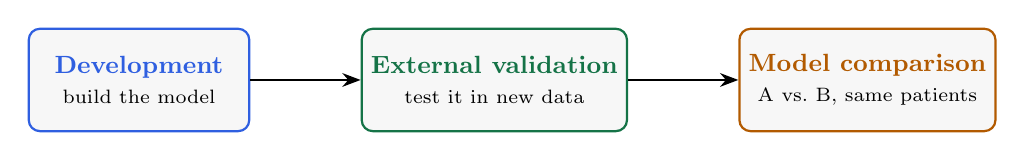
\begin{tikzpicture}[node distance=6mm and 14mm, every node/.style={font=\small},
      box/.style={rounded corners, draw, thick, minimum height=13mm, minimum width=28mm,
                  align=center, fill=black!3}]
    \node[box, draw=devcol] (dev) {\stagechip{devcol}{Development}\\\scriptsize build the model};
    \node[box, draw=valcol, right=of dev] (val) {\stagechip{valcol}{External validation}\\\scriptsize test it in new data};
    \node[box, draw=cmpcol, right=of val] (cmp) {\stagechip{cmpcol}{Model comparison}\\\scriptsize A vs.\ B, same patients};
    \draw[-{Stealth}, thick] (dev) -- (val);
    \draw[-{Stealth}, thick] (val) -- (cmp);
  \end{tikzpicture}
  \vfill
  \begin{columns}[t]
    \column{0.33\textwidth}\footnotesize
      \stagechip{devcol}{Q1.} Is the training set big enough to fit a \emph{stable} model (little overfitting)?
    \column{0.33\textwidth}\footnotesize
      \stagechip{valcol}{Q2/Q3.} Is the validation cohort big enough to estimate performance \emph{precisely}?
    \column{0.33\textwidth}\footnotesize
      \stagechip{cmpcol}{Q4.} Is the cohort big enough to \emph{detect} that model B beats model A?
  \end{columns}
  \vfill
  {\scriptsize This is also the organising logic of TRIPOD+AI (item 10 asks for sample-size justification at development \emph{and} validation).}
\end{frame}

% ---------------------------------------------------------------------
\begin{frame}{Four methods, one timeline}
  \centering
  \begin{tabular}{@{}llll@{}}
    \toprule
    \textbf{Script} & \textbf{Stage} & \textbf{Method paper} & \textbf{Year}\\
    \midrule
    \texttt{ss\_3} & \stagechip{devcol}{Development}         & Riley et al., \emph{BMJ} m441            & 2020\\
    \texttt{ss\_2} & \stagechip{valcol}{Validation (sim.)}   & Snell et al., \emph{J Clin Epidemiol}    & 2021\\
    \texttt{ss\_1} & \stagechip{valcol}{Validation (closed)} & Riley et al.\ (part 3), \emph{BMJ}       & 2023\\
    \texttt{ss\_4} & \stagechip{cmpcol}{Comparison}          & Jung, \emph{Pharm Stat}                  & 2024\\
    \bottomrule
  \end{tabular}
  \vfill
  \begin{block}{Talk order = execution order}
    \stagechip{devcol}{Develop} $\;\rightarrow\;$ \stagechip{valcol}{Validate} (closed form + simulation as a cross-check) $\;\rightarrow\;$ \stagechip{cmpcol}{Compare}.
  \end{block}
\end{frame}

% =====================================================================
\section{Development \quad {\normalsize\texttt{ss\_3} · Riley 2020}}
% =====================================================================
\begin{frame}{Development: four criteria (all reverse-lookup at your $N$)}
  \textbf{Goal:} minimise overfitting \emph{before} you ever validate. Symbols:
  $\varphi$ event fraction, $P$ candidate parameters, $R^2_{cs}$ Cox--Snell $R^2$, $S$ shrinkage.
  \vfill
  \begin{columns}[t]
    \column{0.5\textwidth}
      \begin{block}{B1 --- estimate $\varphi$ precisely}
        $\delta_{\text{margin}} = 1.96\sqrt{\varphi(1-\varphi)/N}$
      \end{block}
      \begin{block}{B2 --- small prediction error (MAPE)}
        \footnotesize$\ln\text{MAPE} = -0.508 - 0.544\ln N + 0.259\ln\varphi + 0.504\ln P$
      \end{block}
    \column{0.5\textwidth}
      \begin{alertblock}{B3 --- shrinkage $S \ge 0.9$ \;(usually binding)}
        $N = \dfrac{P}{(S-1)\,\ln\!\left(1 - R^2_{cs}/S\right)}$
      \end{alertblock}
      \begin{block}{B4 --- optimism in $R^2_{\text{Nagelkerke}} \le 0.05$}
        via $S_{B4}=\dfrac{R^2_{cs}}{R^2_{cs}+\delta\max(R^2_{cs})}$
      \end{block}
  \end{columns}
  \vfill
  {\scriptsize $\max(R^2_{cs}) = 1-\{\varphi^{\varphi}(1-\varphi)^{1-\varphi}\}^2$. \quad Required $N=\max(N_{B1},N_{B2},N_{B3},N_{B4})$.}
\end{frame}

\begin{frame}{Development: what you feed it, what it tells you}
  \begin{columns}[t]
    \column{0.5\textwidth}
      \textbf{Inputs (all scalars --- no CSV needed)}
      \begin{itemize}
        \item $\varphi$: anticipated pCR fraction
        \item $P$: candidate parameters \\ {\scriptsize(fusion models: use a conservative proxy, not the neural-net weight count!)}
        \item $R^2_{cs}$: default $0.15\times\max(R^2_{cs})$
      \end{itemize}
    \column{0.5\textwidth}
      \textbf{Worked example} ($N=717,\ \varphi=0.30,\ P=20$)
      \begin{itemize}
        \item B3 shrinkage $S \approx 0.80$ \textcolor{red}{(target 0.90)}
        \item Required $N \approx \mathbf{1599}$, binding = B3
        \item[$\Rightarrow$] development set \emph{short} $\approx$ 880 patients
      \end{itemize}
  \end{columns}
  \vfill
  \begin{exampleblock}{Takeaway}
    The shrinkage criterion (B3) almost always dominates --- report it as your binding constraint.
  \end{exampleblock}
\end{frame}

% =====================================================================
\section{External validation \quad {\normalsize\texttt{ss\_2}/\texttt{ss\_1} · Snell 2021 / Riley 2023}}
% =====================================================================
\begin{frame}{Validation: from ``required $N$'' to ``achieved precision''}
  Model is \emph{already built}. Question: are the performance estimates in new data \textbf{precise enough}?
  \vfill
  We report the achieved \textbf{95\% CI width} for four measures, against community targets:
  \begin{center}
  \begin{tabular}{@{}lll@{}}
    \toprule
    \textbf{Measure} & \textbf{Target 95\% CI width} & \textbf{Typically\ldots}\\
    \midrule
    $c$-statistic (discrimination)      & $\le 0.10$ & easy to meet\\
    Calibration slope                   & $\le 0.30$ & \alert{the binding one}\\
    O/E ratio (calibration-in-large)    & $\le 0.22$ & moderate\\
    Standardised net benefit            & context     & threshold-specific\\
    \bottomrule
  \end{tabular}
  \end{center}
  \vfill
  {\scriptsize Two engines that should agree: \texttt{ss\_1} closed-form (fast) and \texttt{ss\_2} simulation (flexible).}
\end{frame}

\begin{frame}{\texttt{ss\_1}: closed-form (the \texttt{pmvalsampsize} route)}
  \begin{block}{$c$-statistic --- Newcombe's formula (no iteration)}
    \[
      SE(C)=\sqrt{\frac{C(1-C)\left[1+\left(\tfrac{N}{2}-1\right)\tfrac{1-C}{2-C}+\left(\tfrac{N}{2}-1\right)\tfrac{C}{1+C}\right]}{N^2\varphi(1-\varphi)}}
    \]
  \end{block}
  \begin{columns}[t]
    \column{0.5\textwidth}
      \begin{block}{O/E ratio}
        $SE(\ln O/E)=\sqrt{\dfrac{1-\varphi}{N\varphi}}$
      \end{block}
    \column{0.5\textwidth}
      \begin{block}{Calibration slope}
        Fisher information of $(\alpha,\lambda)$ over the LP distribution (well-calibrated: $\alpha{=}0,\lambda{=}1$).
      \end{block}
  \end{columns}
  \vfill
  {\scriptsize \textbf{Inputs:} $N$, $\varphi$, assumed $c$; optionally a Beta shape for the predicted-risk histogram.}
\end{frame}

\begin{frame}{\texttt{ss\_2}: simulation (Snell 2021) --- when assumptions bite}
  \begin{enumerate}
    \item Assume the linear predictor $LP_i \sim \mathcal{N}(\mu,\sigma^2)$ in the validation population.
    \item Impose a \emph{true} calibration model: $\operatorname{logit}(p_i)=\gamma + S\cdot LP_i$.
      \begin{itemize}\footnotesize
        \item $\gamma=0, S=1$: well calibrated \quad
        \item $S<1$ (e.g.\ 0.9): predictions too extreme --- \emph{stress-test} miscalibration
      \end{itemize}
    \item Simulate $B$ datasets, refit, average the 95\% CI widths.
  \end{enumerate}
  \vfill
  \begin{exampleblock}{Why keep both}
    \texttt{ss\_1} is instant and matches software; \texttt{ss\_2} lets you inject miscalibration and use your
    \emph{real} LP distribution. Agreement between them is a good sanity check.
  \end{exampleblock}
  \vfill
  {\scriptsize Worked example ($N=334$): $c$-width $\approx 0.11$ \textcolor{devcol}{(OK)} but slope width $\approx 0.5$\,--\,0.6 \alert{(wide)} $\Rightarrow$ slope binds.}
\end{frame}

\begin{frame}{Bridge: turning a reported $c$-statistic into $R^2_{cs}$}
  Development (\texttt{ss\_3}) wants $R^2_{cs}$; you often only \emph{have} a $c$-statistic from a pilot/prior model.
  \vfill
  \[
    \delta=\sqrt{2}\,\Phi^{-1}(C)\qquad\Longrightarrow\qquad
    R^2_{cs}\approx 1-\exp\!\left(-\tfrac{\delta^2}{2}\right)\ \text{(approx.)}
  \]
  \vfill
  \begin{alertblock}{Caveat}
    This bridge assumes normal linear predictors --- an \emph{approximation}. Use it as a conservative
    starting point; prefer \texttt{pmsampsize}'s built-in conversion for manuscript numbers.
  \end{alertblock}
\end{frame}

% =====================================================================
\section{Model comparison \quad {\normalsize\texttt{ss\_4} · Jung 2024}}
% =====================================================================
\begin{frame}{Comparing two AUCs on the same patients (paired)}
  Question shifts from ``how good is model B?'' to ``is B \emph{significantly} better than A?''
  --- the sample-size version of \textbf{DeLong's test}.
  \vfill
  \begin{block}{Standardised effect $\leftrightarrow$ AUC}
    $X_k\sim\mathcal N(\delta_k,1)$ (cases), $Y_k\sim\mathcal N(0,1)$ (controls), \quad
    $\theta_k=\Phi\!\left(\delta_k/\sqrt2\right)$
  \end{block}
  \begin{columns}[t]
    \column{0.55\textwidth}
      \begin{block}{Required $N$}
        \[ N=\frac{v\,(z_{1-\alpha/2}+z_{1-\beta})^2}{(\theta_1-\theta_2)^2} \]
        \footnotesize $v=\dfrac{\sigma_1^2+\sigma_2^2-2\sigma_{12}}{\gamma(1-\gamma)}$, computed by numerical integration.
      \end{block}
    \column{0.45\textwidth}
      \begin{block}{Reverse: power at your $N$}
        \[ 1-\beta=\Phi\!\left(\tfrac{\sqrt N\,|\Delta|}{\sqrt v}-z_{1-\alpha/2}\right) \]
      \end{block}
  \end{columns}
  \vfill
  {\scriptsize Key extra input: $\rho$, the correlation between the two models' scores (paired design). Worked: $\theta{=}0.75$ vs $0.82$, $\rho{=}0.5 \Rightarrow N\approx 422$; power at $N{=}334$ only $\approx 0.70$.}
\end{frame}

% =====================================================================
\section{Putting it together}
% =====================================================================
\begin{frame}{What each script needs --- at a glance}
  \centering\small
  \begin{tabular}{@{}llll@{}}
    \toprule
    \textbf{Script} & \textbf{Core question} & \textbf{Key inputs} & \textbf{Key output}\\
    \midrule
    \texttt{ss\_3} & training set big enough?    & $\varphi, P, R^2_{cs}, N$          & required $N$; binding B1--B4\\
    \texttt{ss\_2} & validation precise enough?  & $\mu,\sigma,\gamma,S,N$            & avg 95\% CI widths (sim.)\\
    \texttt{ss\_1} & validation precise enough?  & $\varphi, c, N$                    & achieved 95\% CI widths\\
    \texttt{ss\_4} & B beats A detectable?       & $\theta_1,\theta_2,\rho,\gamma,N$  & required $N$; power; MDD\\
    \bottomrule
  \end{tabular}
  \vfill
  \begin{block}{All four support a \emph{reverse lookup}}
    Plug in your actual cohort size $\rightarrow$ read off achieved precision / power. No guessing $N$ up front.
  \end{block}
\end{frame}

\begin{frame}{Manuscript rationale --- TRIPOD+AI item 10}
  Three drop-in paragraphs (development / validation / comparison). Skeleton:
  \vfill
  \begin{block}{Validation example}
    \footnotesize
    ``Following Riley et al.\ (2023) and, as a sensitivity check, the simulation approach of Snell et al.\ (2021),
    assuming $c=\ldots$ and event proportion $=\ldots$, the $N$ required for 95\% CI widths of
    $\le 0.10$ ($c$), $\le 0.30$ (slope) and $\le 0.22$ (O/E) was $\ldots$ (\ldots events), driven by the
    calibration slope. Our cohort ($N=\ldots$) achieved a slope CI width of $\approx\ldots$, indicating
    [precise / limited] precision.''
  \end{block}
  \vfill
  {\scriptsize The repository ships all three templates ready to fill with your numbers.}
\end{frame}

\begin{frame}{Software: a package + a zero-install web demo}
  \begin{columns}[t]
    \column{0.5\textwidth}
      \textbf{\texttt{sampsizeval} (Python)}
      \begin{itemize}
        \item 4 calculators, one API
        \item CLI: \texttt{sampsizeval dev/val/compare}
        \item CSV $\rightarrow$ parameters ($\varphi, c, \rho$)
        \item \texttt{pytest} test suite
      \end{itemize}
    \column{0.5\textwidth}
      \textbf{Browser demo (Pyodide)}
      \begin{itemize}
        \item Runs 100\% client-side --- data never leaves the machine
        \item Manual inputs \emph{or} drag-in a CSV
        \item Hosted free on GitHub Pages
      \end{itemize}
  \end{columns}
  \vfill
  \begin{exampleblock}{Try it}
    \centering \url{https://csyfjiang.github.io/Sample-Size-Estimation-Tutorial/}
  \end{exampleblock}
\end{frame}

% ---------------------------------------------------------------------
\begin{frame}{Takeaways}
  \begin{enumerate}
    \item Sample size is a \textbf{lifecycle} question: develop $\rightarrow$ validate $\rightarrow$ compare.
    \item Drop the rules of thumb --- required $N$ depends on $\varphi$, $P$, expected performance and \emph{target precision}.
    \item \stagechip{devcol}{Development}: shrinkage (B3) is the usual binding constraint.
    \item \stagechip{valcol}{Validation}: the \emph{calibration slope} CI width usually binds, not the $c$-statistic.
    \item \stagechip{cmpcol}{Comparison}: correlation $\rho$ between models drives the required $N$.
    \item Always report the \textbf{reverse lookup} for your actual cohort (TRIPOD+AI item 10).
  \end{enumerate}
\end{frame}

\begin{frame}[allowframebreaks]{References}
  \footnotesize
  \begin{itemize}
    \item Riley RD, Ensor J, Snell KIE, et al. Calculating the sample size required for developing a
      clinical prediction model. \emph{BMJ} 2020;368:m441.
    \item Snell KIE, Archer L, Ensor J, et al. External validation of clinical prediction models:
      simulation-based sample size calculations were more reliable than rules-of-thumb.
      \emph{J Clin Epidemiol} 2021;135:79--89.
    \item Riley RD, Snell KIE, Archer L, et al. Evaluation of clinical prediction models (part 3):
      calculating the sample size required for an external validation study.
      \emph{BMJ} 2023;383:e074821.
    \item Jung SH. Sample size calculation for comparing two ROC curves.
      \emph{Pharmaceutical Statistics} 2024;23(4):557--569.
    \item van Smeden M, et al. Sample size for binary logistic prediction models.
      \emph{Stat Methods Med Res} 2019.
  \end{itemize}
\end{frame}

\begin{frame}[standout]
  Thank you\\[2mm]
  {\normalsize \url{https://github.com/csyfjiang/Sample-Size-Estimation-Tutorial}}
\end{frame}

\end{document}
